
% use either of the below line graphs:

%\begin{figure}[!th]
%\centering
%\caption{\label{fig:line-pp}Multiple Births Per 1000 Live Births by Mothers' Population Group}
%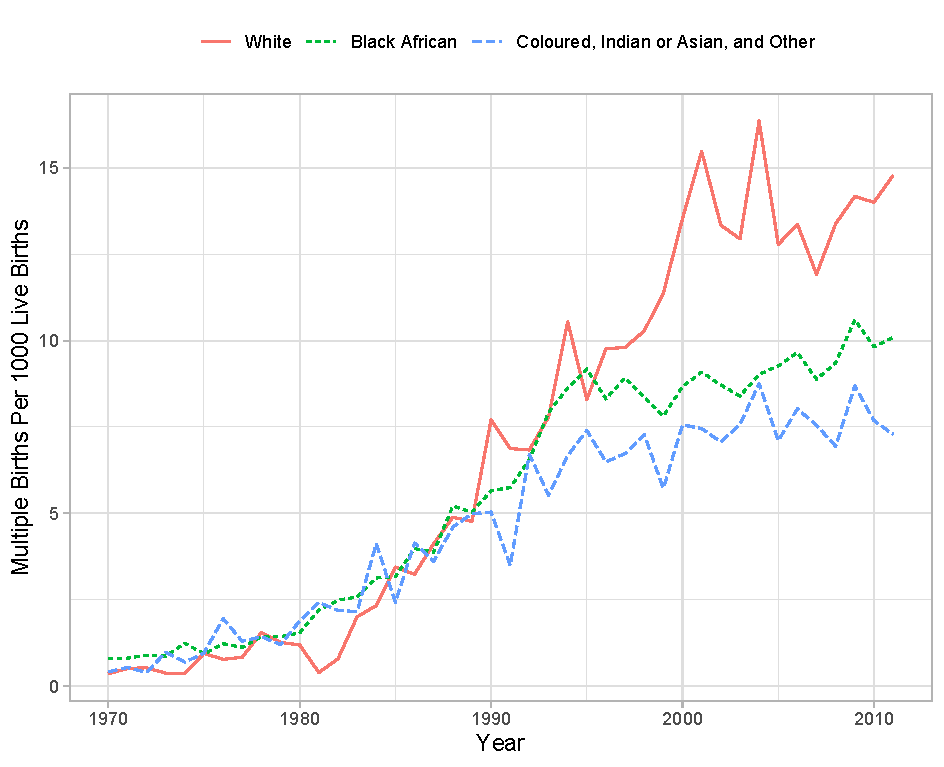
\includegraphics[width=\textwidth]{figures/line_pp.pdf}
%\end{figure}

\begin{figure}[!th]
\centering
\caption{\label{fig:line-pp}Multiple Births Per 1000 Live Births by Mothers' Population Group}
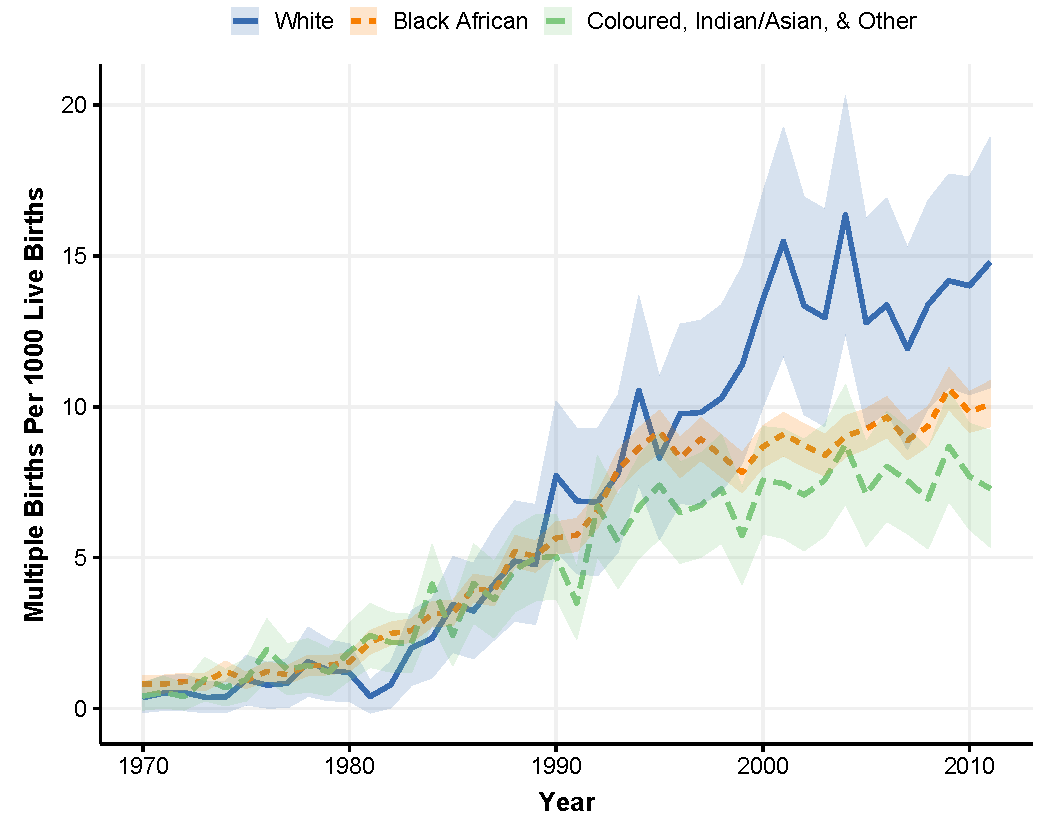
\includegraphics[width=\textwidth]{figures/line_rib.pdf}
\fnote{\textit{Notes:} The solid lines represent the number of multiple births per 1000 live births for each population group, i.e., (number of multiple births/total birth)*1000. The ribbons are point-wise 95\% confidence intervals. The standard errors used to construct the confidence intervals were calculated using the following formula: se $ = 1000 \cdot \sqrt{p\cdot (1 - p)/n} $, where $ p $ is the proportion of multiple birth in a given year and $ n $ is the total number of live births. The formula assumes $ p $ follows the Bernoulli distribution.}
\end{figure}
%\pagebreak


%Tex File: D:/R_projects/MScED_Dissertation/tex/tables/whites-nonwhites.tex

\begin{sidewaystable}[!htbp] \centering 
  \caption{Heterogeneity by Mother's Population Group (Whites vs. Non-Whites)} 
  \label{tab:whites-nonwhites} 
\begin{threeparttable}
\begin{tabular}{@{\extracolsep{8pt}}lcc@{\hskip 0.3in}cc@{\hskip 0.3in}cc@{\hskip 0.3in}cc} 
\\[-1.8ex]\hline 
\hline \\[-1.8ex] 
 & \multicolumn{4}{c}{2+ Sample} & \multicolumn{4}{c}{3+ Sample} \\
\cline{2-5}  \cline{6-9} \\
 & \multicolumn{2}{c}{Whites} & \multicolumn{2}{c}{Non-Whites} & 
    \multicolumn{2}{c}{Whites} & \multicolumn{2}{c}{Non-Whites} \\
\cline{2-3}  \cline{4-5} \cline{6-7} \cline{8-9} \\[-1.8ex]
\\[-1.8ex] & (1) & (2) & (3) & (4) & (5) & (6) & (7) & (8)\\ 
\hline \\[-1.8ex] 
\\[-2.0ex] \multicolumn{9}{@{} l}{\textbf{Panel A: First Stage$^{\dag}$}}
 \\
 \\[-1.5ex]
 Twins2/ & \multicolumn{2}{c}{ 0.942$^{***}$ }  & \multicolumn{2}{c}{ 0.809$^{***}$ } 
  &  \multicolumn{2}{c}{ 0.861$^{***}$ }  &  \multicolumn{2}{c}{ 0.756$^{***}$ }  \\ 
 Twins3 & \multicolumn{2}{c}{ (0.044) }  & \multicolumn{2}{c}{ (0.030) } 
  &  \multicolumn{2}{c}{ (0.068) }  &  \multicolumn{2}{c}{ (0.037) }  \\ 
 \multicolumn{1}{c}{$F$}  & \multicolumn{2}{c}{ [447.7] } & \multicolumn{2}{c}{ [732.5] } & \multicolumn{2}{c}{ [162.9] } & \multicolumn{2}{c}{ [422.2] } \\
\\[-1.83ex] 
 \hline \\[-1.83ex]
\\[-2.0ex] \multicolumn{9}{@{} l}{\textbf{Panel B: OLS \& 2SLS$^{\ddag}$}}
 \\
 \\[-1.5ex]
 & OLS & IV & OLS & IV & OLS & IV & OLS & IV \\
 \hline \\
 Educational Attainment & $-$0.001 & 0.019 & $-$0.005$^{***}$ & 0.003 & $-$0.009 & 0.026 & $-$0.007$^{***}$ & 0.011 \\ 
  & (0.002) & (0.012) & (0.001) & (0.007) & (0.005) & (0.018) & (0.001) & (0.010) \\ 
  & & & & & & & & \\ 
 Left Behind & 0.018$^{*}$ & $-$0.034 & 0.020$^{***}$ & $-$0.001 & 0.023 & $-$0.009 & 0.024$^{***}$ & $-$0.025 \\ 
  & (0.009) & (0.042) & (0.002) & (0.021) & (0.020) & (0.082) & (0.003) & (0.027) \\ 
  & & & & & & & & \\ 
 Private School & 0.021$^{**}$ & $-$0.010 & $-$0.004$^{***}$ & $-$0.017 & 0.047$^{*}$ & $-$0.094 & $-$0.004$^{***}$ & 0.015 \\ 
  & (0.007) & (0.035) & (0.001) & (0.011) & (0.019) & (0.081) & (0.001) & (0.015) \\ 
  & & & & & & & & \\ 
 Mothers LFP & $-$0.016$^{**}$ & 0.008 & $-$0.020$^{***}$ & $-$0.024 & $-$0.009 & 0.044 & $-$0.023$^{***}$ & 0.040 \\ 
  & (0.006) & (0.027) & (0.002) & (0.018) & (0.019) & (0.080) & (0.003) & (0.032) \\ 
  & & & & & & & & \\ 
\hline \\[-1.8ex] 
 $ N $  & \multicolumn{2}{c}{10,121} & \multicolumn{2}{c}{84,856} & \multicolumn{2}{c}{3,494} & \multicolumn{2}{c}{53,864} \\
\\[-2.0ex]
\hline 
\hline \\[-1.8ex] 
\end{tabular} 
\begin{tablenotes}
\footnotesize
\item \textit{Notes:} *** Significant at 1\%, ** Significant at 5\%, * Significant at 10\%. \\[-1.8ex] 

$ \dag $ Columns 1-4 have the coefficients for the Twins2
instrument (in the 2+ sample) and in columns 5-8 are the coefficients for the
Twins3 instrument (3+ sample). The regressions were run using the same set 
of controls as in \autoref{tab:main-res}. Robust standard errors are in parentheses and the numbers 
in square brackets below the s.e. are F stats for the exclusion of the Twins2 or
the Twins 3 variable from the model. \\[-1.8ex]
 
$ \ddag $ The regressions control for the same set of covariates as in \autoref{tab:main-res} (see notes there). 
The regressions for the 3+ sample are clustered by mother's ID. 

\end{tablenotes}
\end{threeparttable}
\end{sidewaystable} 



 
\pagebreak


%Tex File: D:/R_projects/MScED_Dissertation/tex/tables/reduced.tex

\begin{table}[!htbp] \centering 
  \caption{Reduced Form Effects in No-First-Stage Samples} 
  \label{tab:reduced} 
\begin{threeparttable}
\begin{tabular}{@{\extracolsep{5pt}}lcccc} 
\\[-1.8ex]\hline 
\hline \\[-1.8ex] 
 & \multicolumn{2}{c}{Twins2$^{\dag}$} & \multicolumn{2}{c}{Boy12$^{\ddag}$} \\
 \cline{2-3} \cline{4-5} \\
 & Spacing $<$ 2 & No Schooling & Spacing $<$ 2 & No Schooling \\
\\[-1.8ex] & (1) & (2) & (3) & (4)\\ 
\hline \\[-1.8ex] 
\\[-2.0ex] \multicolumn{5}{@{} l}{\textbf{Panel A: First Stage}}
 \\
 \\[-1.5ex]
 No. of children & 0.266$^{*}$ & 0.101 & $-$0.0004 & 0.041 \\ 
  & (0.141) & (0.134) & (0.037) & (0.046) \\ 
  & & & & \\ 
\\[-1.83ex] 
 \hline \\[-1.83ex]
\\[-2.0ex] \multicolumn{5}{@{} l}{\textbf{Panel B: Reduced Form$^{\S}$}}
 \\
 \\[-1.5ex]
 Educational Attainment & 0.031 & 0.006 & 0.001 & 0.007 \\ 
  & (0.025) & (0.021) & (0.006) & (0.007) \\ 
  & & & & \\ 
 Left Behind & $-$0.131$^{*}$ & $-$0.067 & 0.013 & $-$0.026 \\ 
  & (0.070) & (0.067) & (0.018) & (0.020) \\ 
  & & & & \\ 
 Private School & 0.027 & $-$0.011$^{***}$ & 0.005 & 0.001 \\ 
  & (0.053) & (0.004) & (0.011) & (0.006) \\ 
  & & & & \\ 
 Mothers LFP & 0.033 & $-$0.052 & 0.034$^{**}$ & 0.005 \\ 
  & (0.065) & (0.067) & (0.015) & (0.020) \\ 
  & & & & \\ 
\hline \\[-1.8ex] 
 $ N $  & 3,489 & 3,022 & 2,869 & 2,381 \\
\hline 
\hline \\[-1.8ex] 
\end{tabular} 
\begin{tablenotes}
\footnotesize
\item \textit{Notes:} *** Significant at 1\%, ** Significant at 5\%, * Significant at 10\%. 
The same set of covariates as in \autoref{tab:main-res} were included in all regressions. Robust standard
errors in parentheses.
\\[-1.8ex]

$ \dag $ The subsamples are restricted to firstborns from families with at least three children.

$ \ddag $ Subsamples includes only firstborn boys.

$ \S $ In addition to the covariates used in \autoref{tab:main-res}, the reduced form regressions control for 
the number of children in the family.
\end{tablenotes}
\end{threeparttable}
\end{table} 




%\pagebreak

